\chapter{Organisation d'un document}
\label{chap:organisation}


\section{Choix d'une classe}
\label{sec:organisation:classe}

La toute première chose à faire au moment de se lancer dans la
rédaction d'un document avec {\LaTeX} consiste normalement à choisir
une classe pour celui-ci. Nous avons déjà expliqué à la
\autoref{sec:bases:classes} comment spécifier la classe à utiliser
et les diverses options; la présente section détaille les différences
entre les principales classes.

Les classes standards sont \class{article}, \class{report},
\class{book}, \class{letter} et \class{slides}.

\begin{description}
\item[\normalfont\class{article}] Articles scientifiques et autres
  documents de longueur modérée ne nécessitant pas une mise en page
  élaborée. Le folio\footnote{Numéro de page} est placé au centre du
  pied de page. Le titre apparait dans le haut de la première page,
  immédiatement suivi du texte.
\item[\normalfont\class{report}] Rapports et autres documents plus
  longs pouvant être divisés en chapitres. Le titre apparait sur une
  page de titre. La mise en page est autrement identique à celle de la
  classe \class{article}.
\item[\normalfont\class{book}] Longs documents divisés en chapitres.
  La mise en page est conçue pour une impression recto-verso. L'entête
  de la page (autre que la première du chapitre) contient le folio sur
  le bord extérieur et le titre de chapitre (page paire) ou le titre
  de section (page impaire). Le titre apparait sur une page de titre.
\item[\normalfont\class{letter}] Lettres et correspondance. Bien que
  puissante, cette classe est plus rarement utilisée. Nous n'en traitons
  pas davantage dans ce document.
\item[\normalfont\class{slides}] Diapositives simples pour des
  présentations. La \autoref{sec:trucs:diapositives} traite plus en
  détail de la production de diapositives.
\end{description}

On trouvera un sommaire des principales caractéristiques des classes
\class{article}, \class{report} et \class{book} dans le
\autoref{tab:organisation:classes}. De plus, les figures
\ref{fig:organisation:classes:article}--\ref{fig:organisation:classes:book}
fournissent des exemples de mise en page pour ces trois classes.

\begin{table}
  \caption{Caractéristiques des principales classes standards}
  \label{tab:organisation:classes}
  \begin{tabularx}{1.0\linewidth}{XXXXX}
    \toprule
    Classe & Divisions & Disposition & Entête & Pied de page \\
    \midrule
    \class{article} & parties,\newline sections, \dots
                       & recto & vide & folio centré \\
    \addlinespace[6pt]
    \class{report} & parties,\newline chapitres,\newline sections, \dots
                       & recto & vide & folio centré \\
    \addlinespace[6pt]
    \class{book} & parties,\newline chapitres,\newline sections, \dots
                       & recto-verso & folio, titres & vide \\
    \bottomrule
  \end{tabularx}
\end{table}

\begin{figure}
  \begin{minipage}{0.48\linewidth}
    \fbox{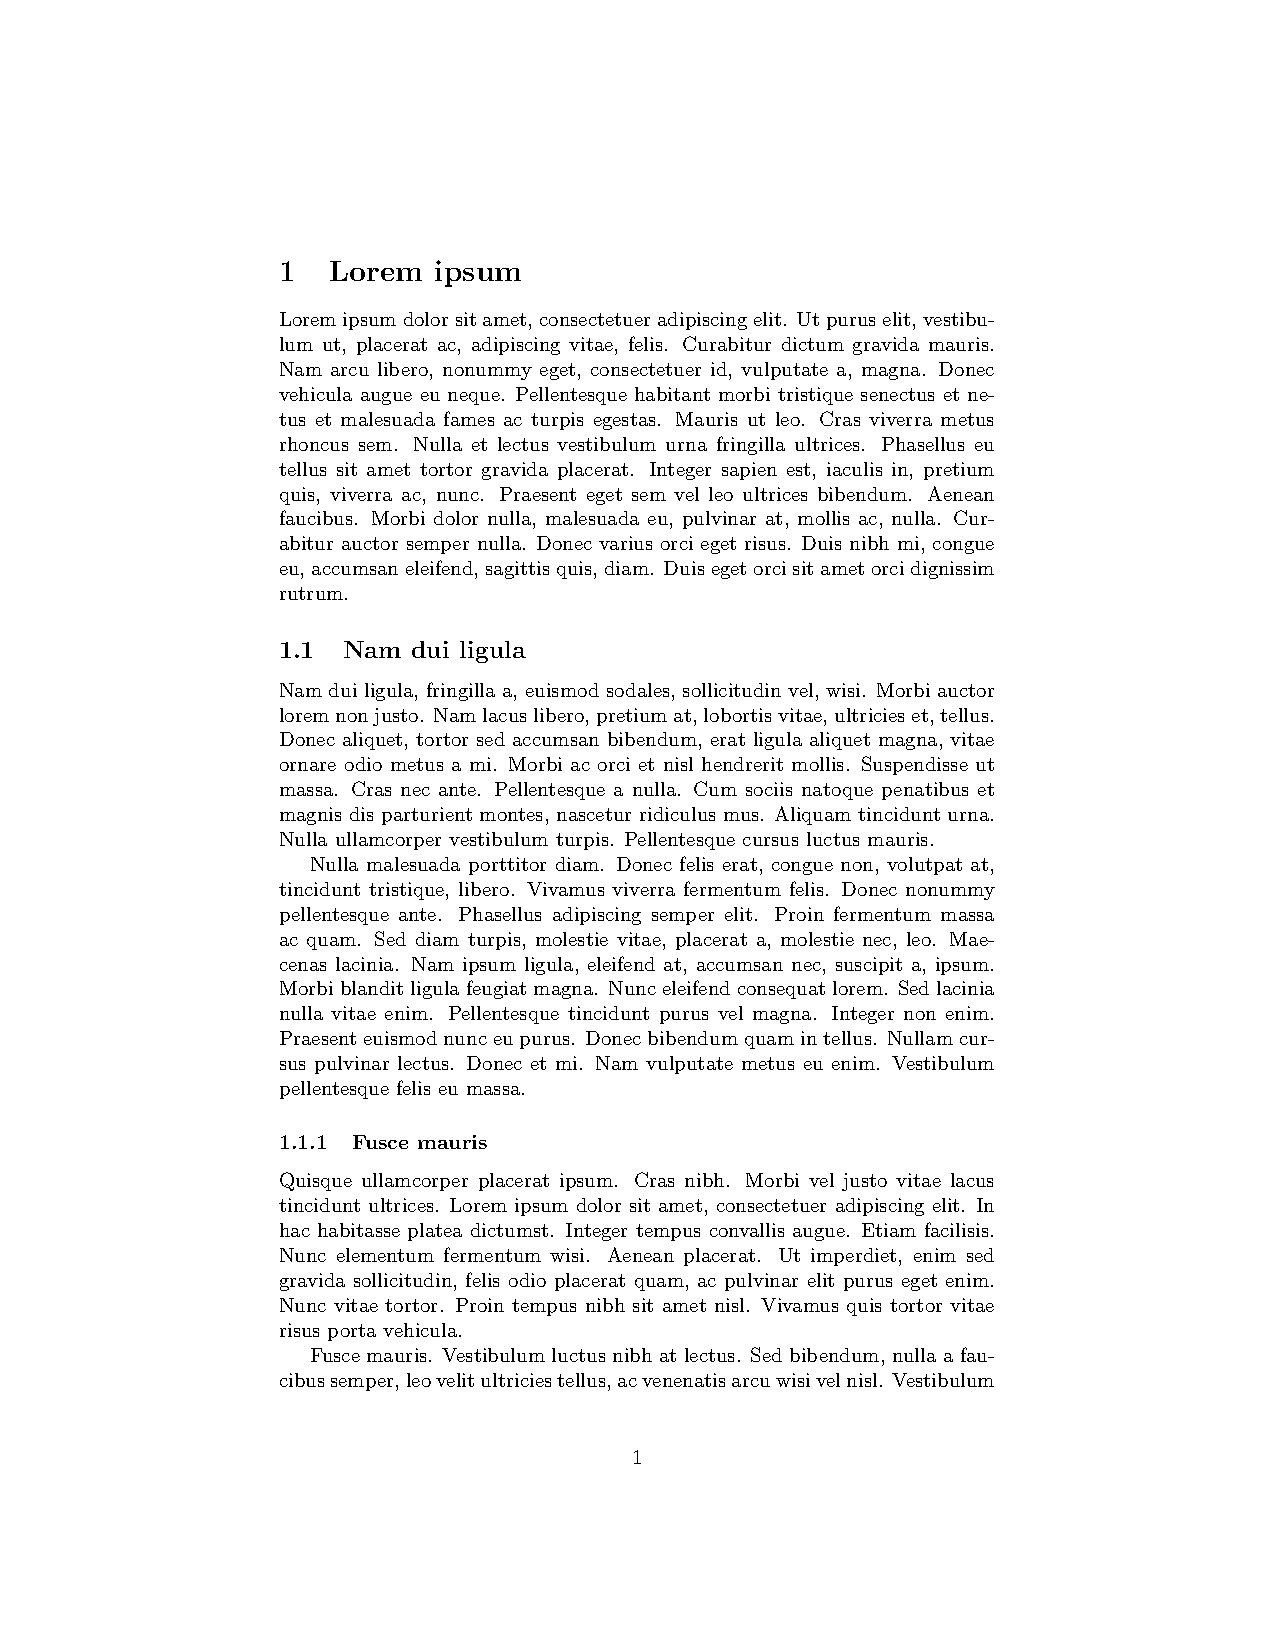
\includegraphics[page=1,width=\linewidth]{exemple-classe-article}}
  \end{minipage}
  \hfill
  \begin{minipage}{0.48\linewidth}
    \fbox{\includegraphics[page=2,width=\linewidth]{exemple-classe-article}}
  \end{minipage}
  \caption{Exemple de mise en page avec la classe \class{article}}
  \label{fig:organisation:classes:article}
\end{figure}

\begin{figure}
  \begin{minipage}{0.48\linewidth}
    \fbox{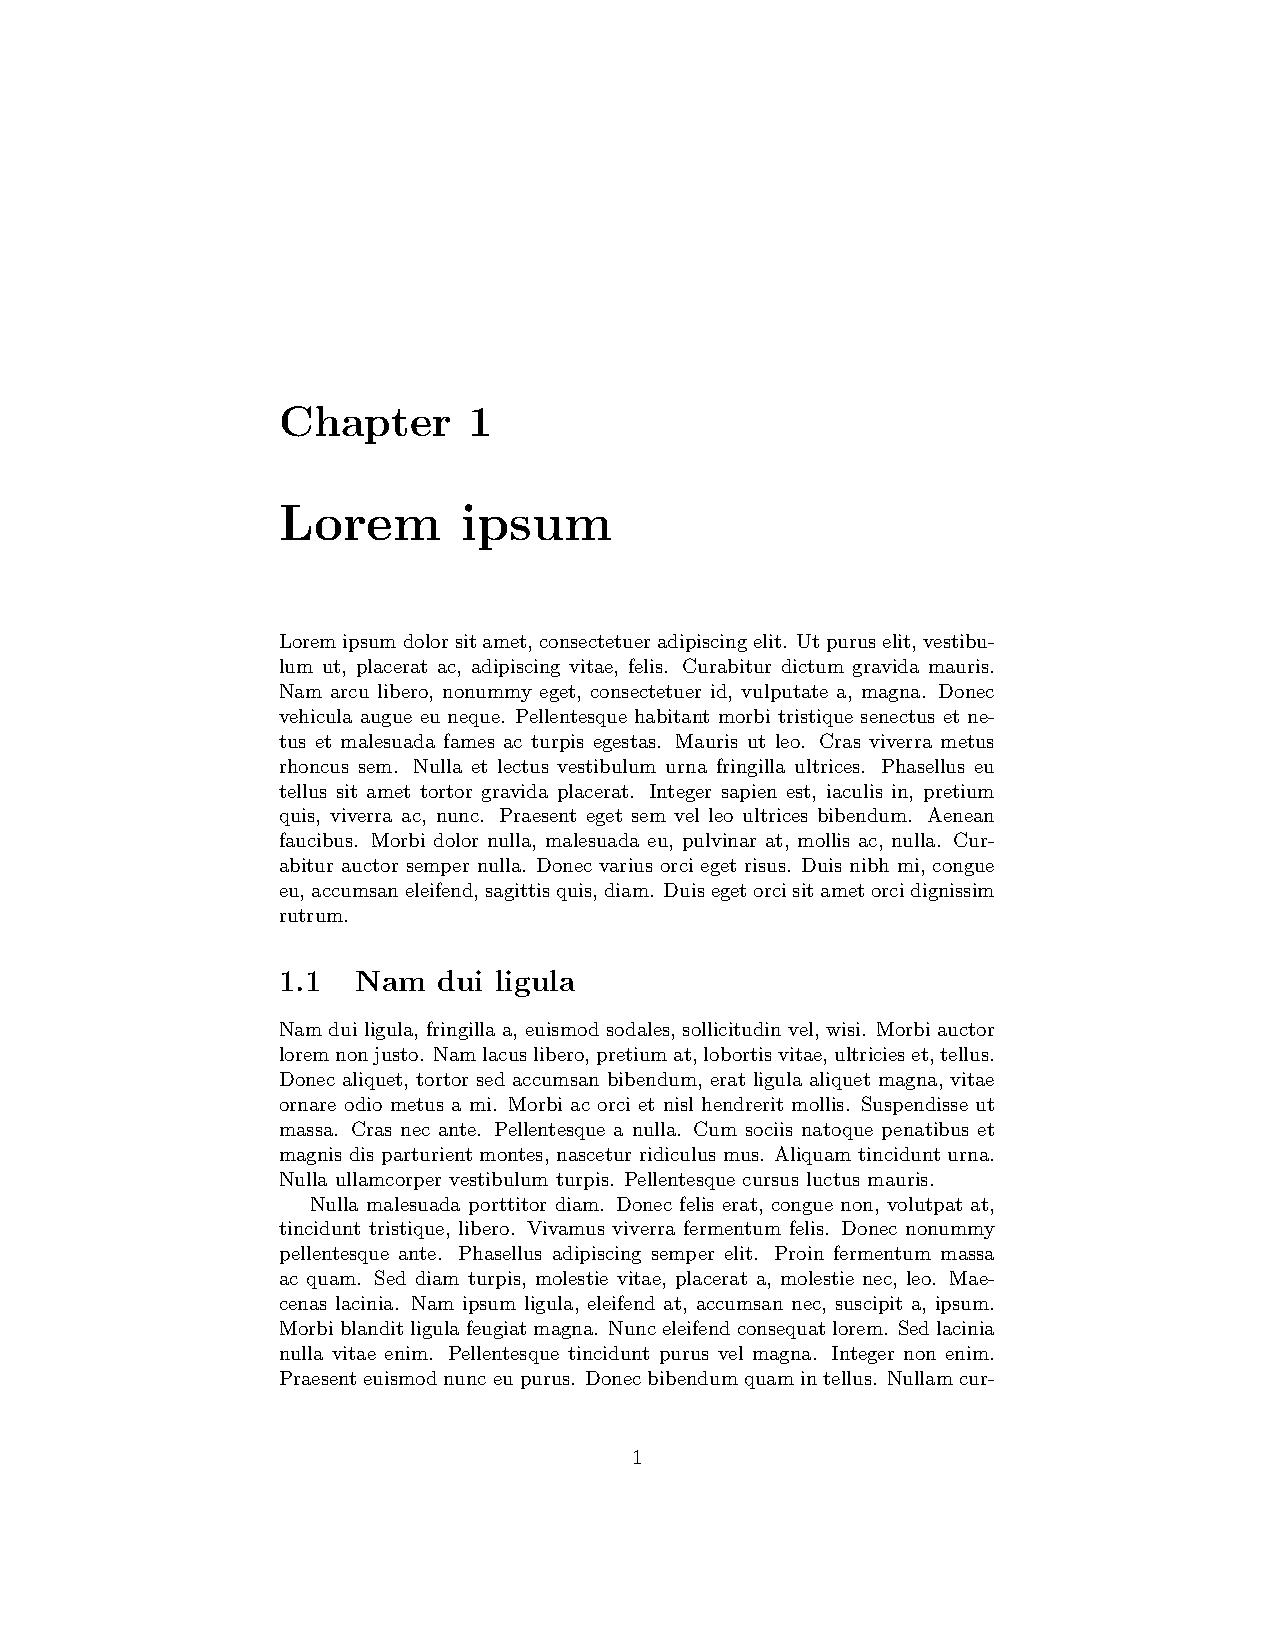
\includegraphics[page=1,width=\linewidth]{exemple-classe-report}}
  \end{minipage}
  \hfill
  \begin{minipage}{0.48\linewidth}
    \fbox{\includegraphics[page=2,width=\linewidth]{exemple-classe-report}}
  \end{minipage}
  \caption{Exemple de mise en page avec la classe \class{report}}
  \label{fig:organisation:classes:report}
\end{figure}

\begin{figure}
  \begin{minipage}{0.48\linewidth}
    \fbox{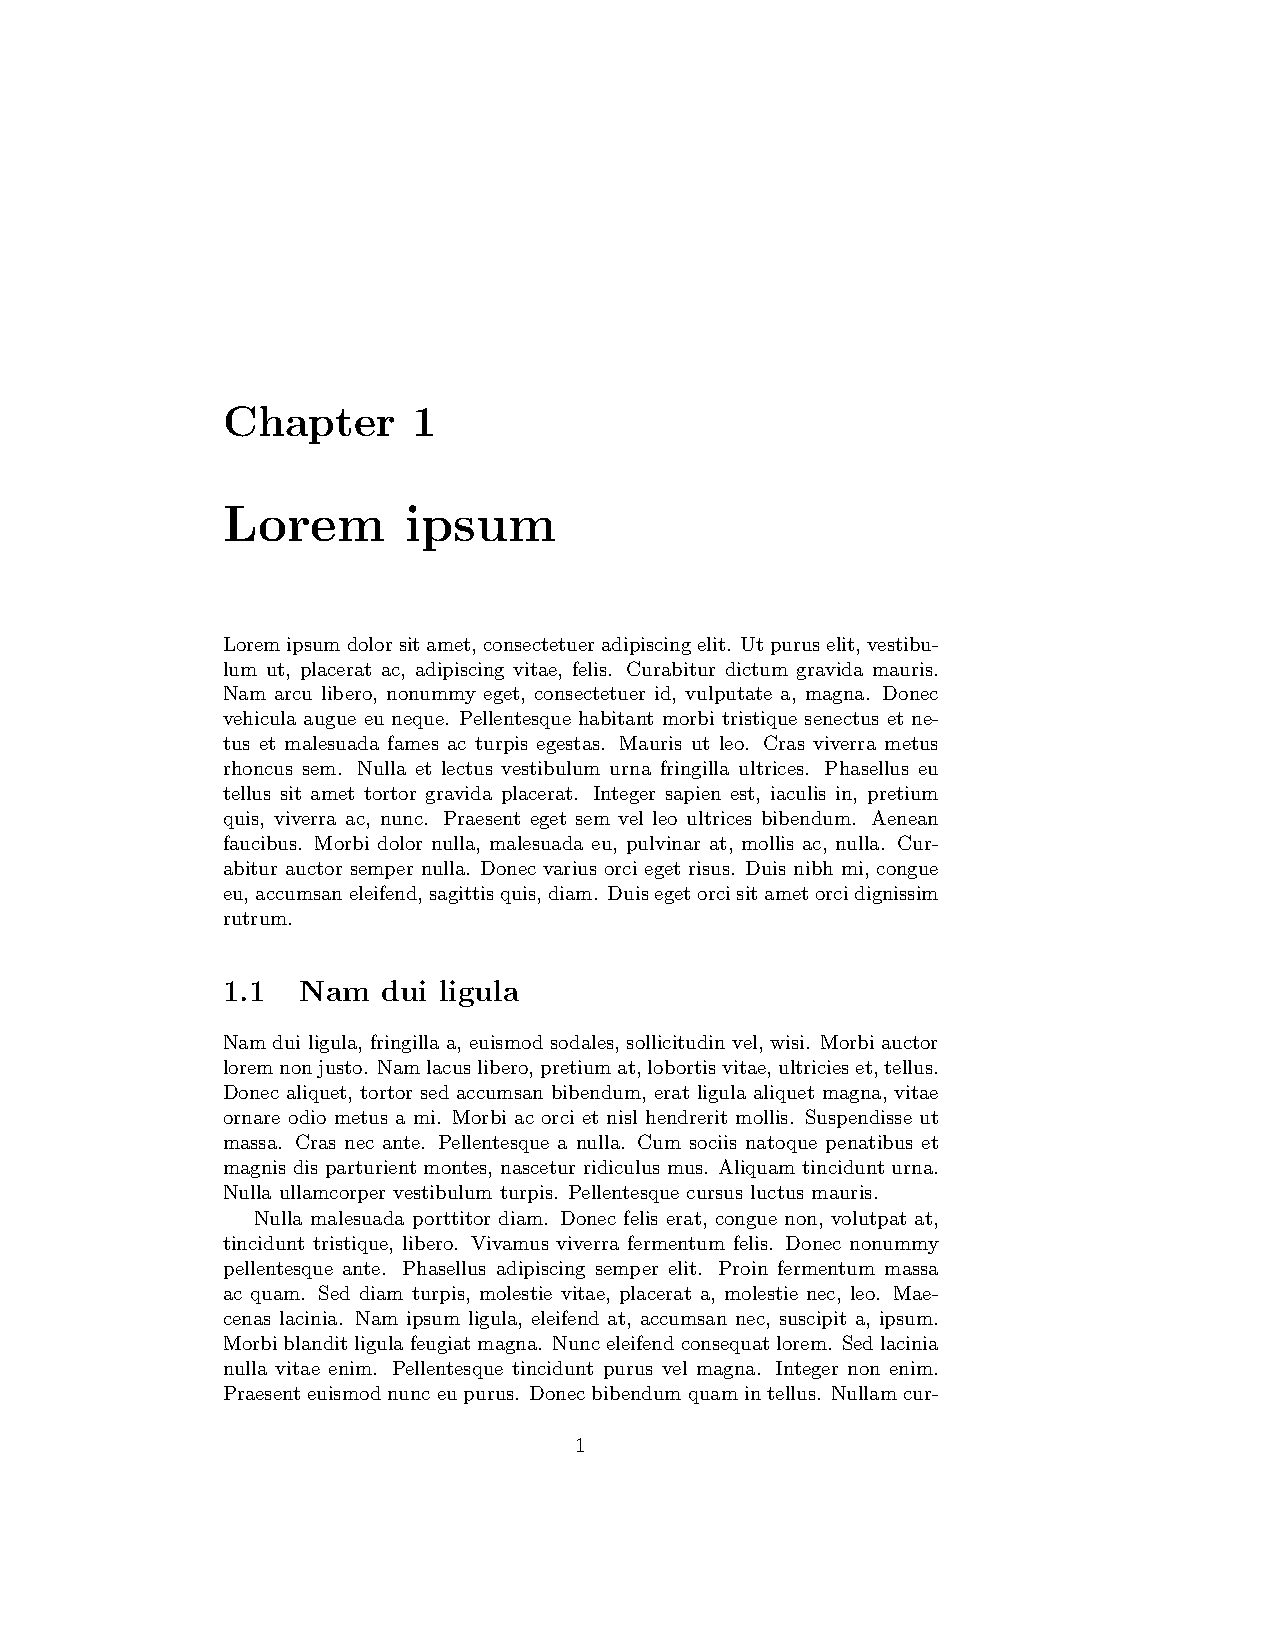
\includegraphics[page=1,width=\linewidth]{exemple-classe-book}}
  \end{minipage}
  \hfill
  \begin{minipage}{0.48\linewidth}
    \fbox{\includegraphics[page=2,width=\linewidth]{exemple-classe-book}}
  \end{minipage}
  \caption{Exemple de mise en page avec la classe \class{book}}
  \label{fig:organisation:classes:book}
\end{figure}

Ce document fait une large place à la classe \class{memoir}, une
extension de la classe standard \class{book} qui facilite à plusieurs
égards la préparation de documents d'allure professionnelle dans
{\LaTeX}. Nous recommandons d'utiliser cette classe en lieu et place
de la classe \class{book}, ou même de la classe \class{article} (voir
ci-dessous).

La classe \class{memoir} est très configurable et elle incorpore
d'office plus de 30 des paquetages les plus populaires\footnote{%
  Consulter la section~18.24 de la documentation de \class{memoir}
  pour la liste ou encore le fichier journal (\emph{log}) de la
  compilation d'un document utilisant la classe.}. %
Comme la classe fait partie des distributions {\LaTeX} modernes, elle
devrait être installée et disponible sur votre système. Elle est
livrée avec une %
\doc{memman}{http://texdoc.net/pkg/memoir} %
exhaustive: le manuel d'instructions fait près de 600~pages! Il peut
être utile de s'y référer de temps à autre pour réaliser une mise en
page particulière.

Les auteurs d'un mémoire ou d'une thèse déposé à l'Université Laval
doivent utiliser la classe \class{ulthese} \citep{ulthese}. Celle-ci
est basée sur la classe \class{memoir}. Par conséquent, toutes les
fonctionnalités de \class{memoir} se retrouvent dans \class{ulthese}.

On rappelle que l'on charge une classe de document au début du
préambule avec la commande
\begin{lstlisting}
\documentclass`\oarg{options}\marg{classe}'
\end{lstlisting}
Les \meta{options} disponibles varient d'une classe à l'autre. Les
plus courantes sont les suivantes.
\begin{description}
\item[\mdseries \code{10pt}, \code{11pt}, \code{12pt}] Taille de la
  police du document en points. La valeur par défaut est \code{10pt}.
  Nous recommandons d'utiliser plutôt \code{11pt}. C'est d'ailleurs la
  taille par défaut avec la classe \class{ulthese}.
\item[\mdseries \code{oneside}, \code{twoside}] Disposition du
  document en recto seulement ou en recto-verso. Ces options ne sont
  utiles que pour modifier la disposition par défaut de la classe. Les
  thèses et mémoire de l'Université Laval sont produits en recto
  seulement.
\item[\mdseries \code{openright}, \code{openany}] Position de la
  première page des chapitres toujours à droite (page impaire) ou
  immédiatement après la dernière page du chapitre précédent. Avec la
  valeur par défaut, \code{openany}, {\LaTeX} insérera une page
  blanche dans le document si un chapitre se termine sur une page
  impaire.
\item[\mdseries \code{article}] Mise en page comme celle d'un article
  (classe \class{memoir} seulement). Avec cette option, \class{memoir}
  peut remplacer la classe \class{article}.
\end{description}


\section{Titre et page de titre}

\begin{itemize}
\item Mise en forme automatique
\begin{lstlisting}
%% préambule
\title`\marg{Titre du document}'
\author`\marg{Prénom Nom}'
\date`\marg{1{\ier} janvier 1970}' % automatique si omis

option titlepage avec classe article

%% corps du document
\maketitle
\end{lstlisting}
\item Mise en forme libre
  \begin{minipage}{0.45\linewidth}
    classes standards
\begin{lstlisting}
\begin{titlepage}
  ...
\end{titlepage}
\end{lstlisting}
  \end{minipage}
  \hfill
  \begin{minipage}{0.45\linewidth}
    classe \class{memoir}
\begin{lstlisting}
\begin{titlingpage}
  ...
\end{titlingpage}
\end{lstlisting}
  \end{minipage}
\end{itemize}

\section{Résumé}

\begin{itemize}
\item Classes \class{article}, \class{report} ou \class{memoir}:
  résumé créé avec l'environnement
\begin{lstlisting}
\begin{abstract}

\end{abstract}
\end{lstlisting}
\item Classe \class{ulthese}: résumés français et anglais traités
  comme des chapitres normaux (non numérotés).
\end{itemize}


\section{Table des matières}

\begin{itemize}
\item Table des matières produite automatiquement avec
\begin{lstlisting}
\tableofcontents
\end{lstlisting}
\item Requiert plusieurs compilations
\item Sections non numérotées pas incluses
\item Avec \pkg{hyperref}, produit également la table des matières du
  fichier PDF
\item Classe \class{memoir} fournit également
\begin{lstlisting}
\tableofcontents*
\end{lstlisting}
  qui n'insère pas la table des matières dans la table des matières
\item Aussi disponibles:
\begin{lstlisting}
\listoffigures
\listoftables
\end{lstlisting}
  (et leurs versions \verb=*= dans \class{memoir})
\end{itemize}


\section{Sections}

\begin{itemize}
\item Découpage du document en sections avec les commandes
\begin{lstlisting}
\part`\marg{titre}'
\chapter`\marg{titre}'
\section`\marg{titre}'
\subsection`\marg{titre}'
\subsubsection`\marg{titre}'
\paragraph`\marg{titre}'
\end{lstlisting}
\item Prennent le titre en argument
\item Numérotation automatique
\item Commande suivie d'une \verb=*= = section non numérotée
\item Éviter d'utiliser des sous-sous-sections
  (\cmdprint{\subsubsection}) dans un livre puisque cela résulte en
  une numérotation à quatre niveaux qui s'avère difficile à suivre pour le
  lecteur.
\item Nous n'avons jamais utilisé le niveau de division \cmdprint{\paragraph}.
\end{itemize}


\section{Annexes}

\begin{itemize}
\item Les annexes sont des sections ou des chapitres avec une
  numérotation alphanumérique (A, A.1, ...)
\item Sections suivantes identifiées comme des annexes par la commande
\begin{lstlisting}
\appendix
\end{lstlisting}
\item Dans le titre, «Chapitre» changé pour «Annexe» le cas échéant
\end{itemize}


\section{Structure logique d'un livre}


\begin{lstlisting}
\frontmatter
\end{lstlisting}
\begin{itemize}
\item préface, table des matières, etc.
\item numérotation des pages en chiffres romains (i, ii, ...)
\item chapitres non numérotés
\end{itemize}

\begin{lstlisting}
\mainmatter
\end{lstlisting}
\begin{itemize}
\item le contenu à proprement parler
\item numérotation des pages à partir de 1 en chiffres arabes
\item chapitres numérotés
\end{itemize}

\begin{lstlisting}
\backmatter
\end{lstlisting}
\begin{itemize}
\item tout le reste (bibliographie, index, etc.)
\item numérotation des pages se poursuit
\item chapitres non numérotés
\end{itemize}


\section{Renvois automatiques}
\label{sec:construction:renvois}


\subsection{Étiquettes et renvois}

Parce que l'ordinateur le fera mieux que vous

\begin{itemize}
\item Ne \emph{jamais} renvoyer manuellement à un numéro de section,
  d'équation, de tableau, etc.
\item «Nommer» un élément avec \verb=\label=
\item Faire référence par son nom avec \verb=\ref=
\item Requiert 2 à 3 compilations
\end{itemize}

\begin{demo}
\begin{lstlisting}[emph={\label,\ref}]
\section{Définitions}
\label{sec:definitions}

Lorem ipsum dolor sit amet, consectetur
adipiscing elit. Duis in auctor dui. Vestibulum

\section{Historique}

Tel que vu à la section \ref{sec:definitions},
on a...
\end{lstlisting}
  \begin{framed}
    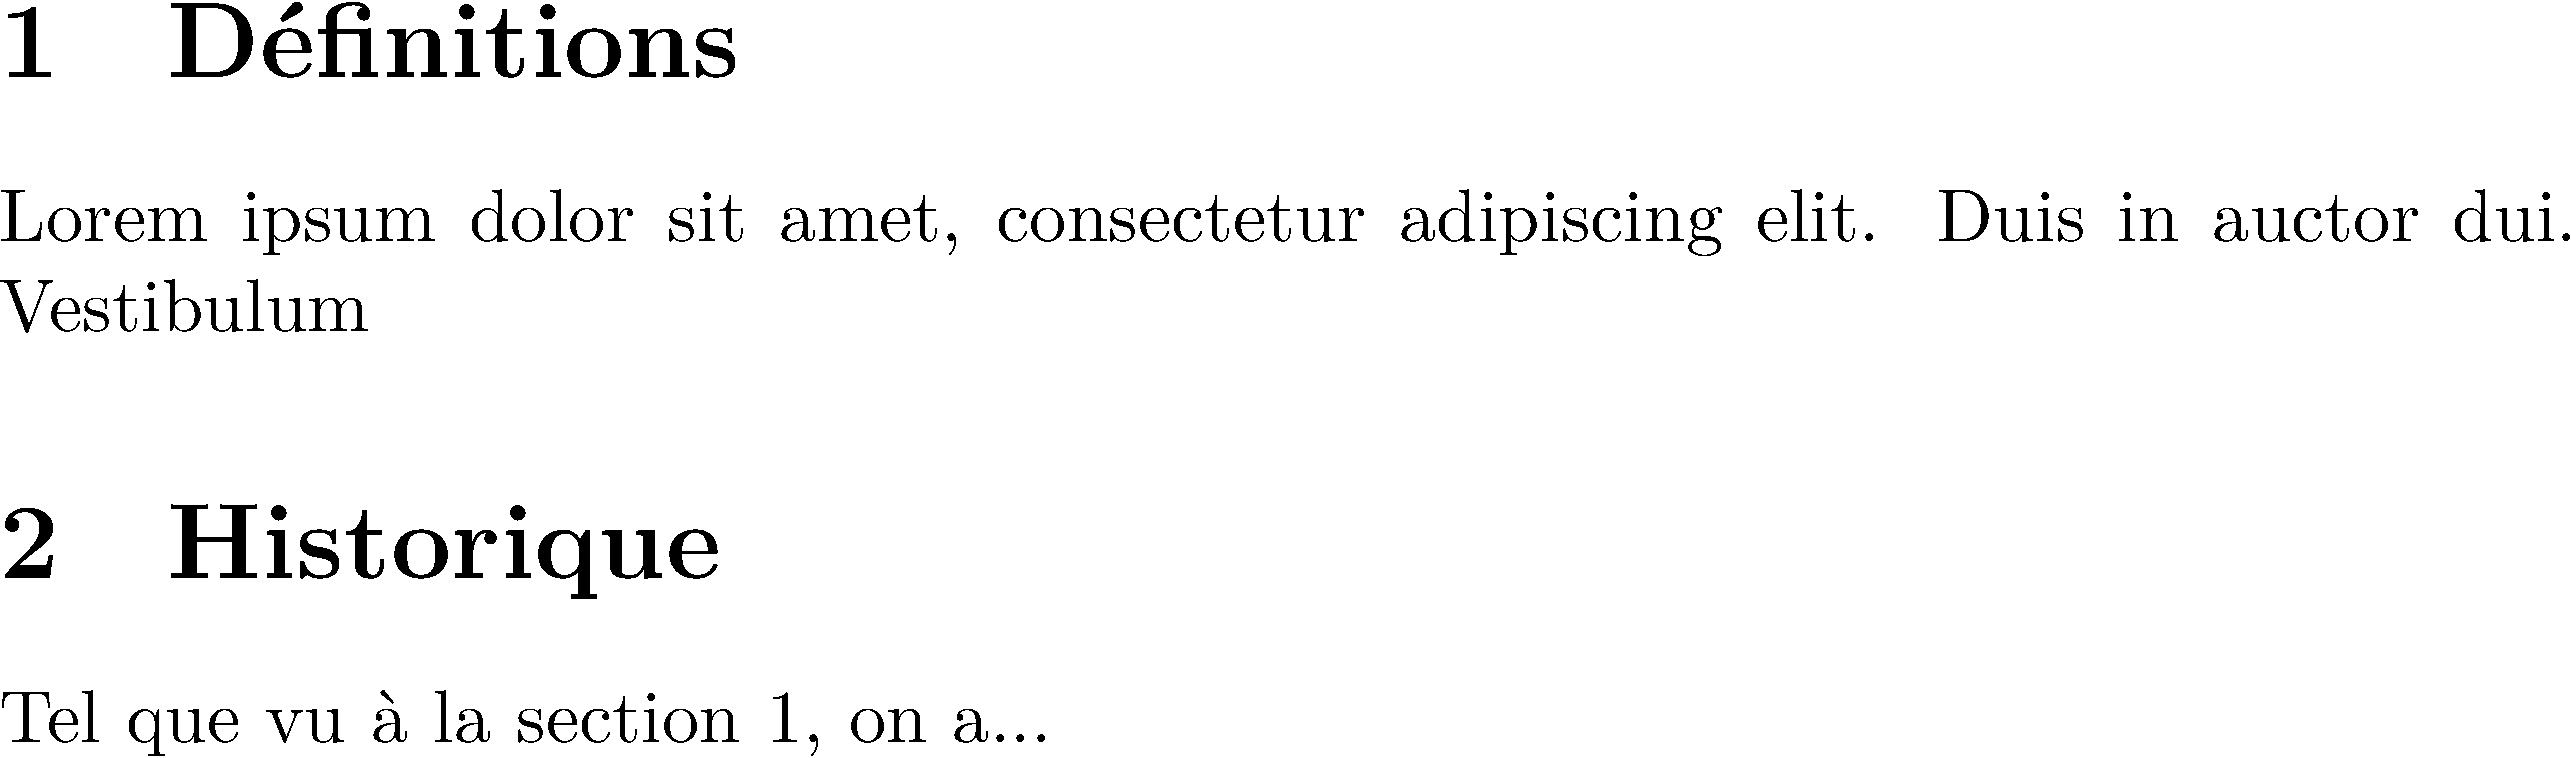
\includegraphics[width=\linewidth]{renvoi}
  \end{framed}
\end{demo}

\begin{conseil}
  Adoptez une manière systématique et mnémotechnique de nommer les
  éléments dans un long document afin de vous y retrouver.

  \bigskip %
  Exemple:
\begin{lstlisting}
\label{chap:`\meta{chapitre}'}          % chapitre
\label{sec:`\meta{chapitre}':`\meta{section}'}  % section
\label{tab:`\meta{chapitre}':`\meta{tableau}'}  % tableau
\label{eq:`\meta{chapitre}':`\meta{equation}'}  % équation
\end{lstlisting}
\end{conseil}


\subsection{Hyperliens}

Renvois automatiques++

\begin{itemize}
\item Paquetage \pkg{hyperref} insère des hyperliens vers les renvois
  dans les fichiers PDF
  \begin{demo}
\begin{lstlisting}
Tel que vu à la section \ref{sec:definitions},
on a...
\end{lstlisting}
    \begin{framed}
      
\includegraphics{renvoi_avec_ref}
    \end{framed}
  \end{demo}
\item Commande \verb=\autoref= permet de
  \begin{enumerate}
  \item nommer automatiquement le type de renvoi (section, équation,
    tableau, etc.)
  \item transformer en hyperlien le texte \textbf{et} le numéro
  \end{enumerate}
  \begin{demo}
\begin{lstlisting}
Tel que vu à la \autoref{sec:definitions},
on a...
\end{lstlisting}
    \begin{framed}
      
\includegraphics{renvoi_avec_autoref}
    \end{framed}
  \end{demo}
\end{itemize}




%%%
%%% Exercices
%%%

\section{Exercices}
\label{sec:apparence:exercices}

\begin{exercice}[nosol]
  Utiliser le fichier \fichier{exercice\_parties.tex}.
  \begin{enumerate}
  \item Étudier la structure du document dans le code source.
  \item Ajouter un titre et un auteur au document.
  \item Créer la table des matières du document en le compilant 2 à 3
    fois.
  \item Insérer deux ou trois titres de sections de différents niveaux
    dans le document.
  \item Vous remarquerez que la numérotation cesse à partir des
    sous-sections. C'est une particularité de la classe
    \class{memoir}.

    Recompiler le document après avoir ajouté au préambule la commande
\begin{lstlisting}
\maxsecnumdepth{subsection}
\end{lstlisting}
  \item Ajouter une annexe au document.
  \end{enumerate}
\end{exercice}

\begin{exercice}[nosol]
  Utiliser le fichier \fichier{exercice\_renvois.tex}.
  \begin{enumerate}
  \item Insérer dans le texte un renvoi au numéro d'une section.
  \item Activer le paquetage \pkg{hyperref} avec l'option
    \code{colorlinks} et comparer l'effet d'utiliser \cmd{\ref} ou
    \cmd{\autoref} pour le renvoi.
  \end{enumerate}
\end{exercice}


%%% Local Variables:
%%% mode: latex
%%% TeX-engine: xetex
%%% TeX-master: "formation-latex-ul"
%%% coding: utf-8
%%% End:
